The two constants for this method of experiment are the mass of the connecting rod which is weighted to be 2.65 kg $\pm$ 0.1 kg and the length of the connecting rod which has a length of 0.33 m $\pm$ 0.001 m. \\

The two trials experimental results are shown on the table below where the first trial will the period of natural oscillations at point A and the second trials will the period of natural oscillations at point B. In addition that, each trials are repeated thrice as suggested by the laboratory guide. The experimental setup is shown on the figure below:\\
\begin{figure}[H]
\centering
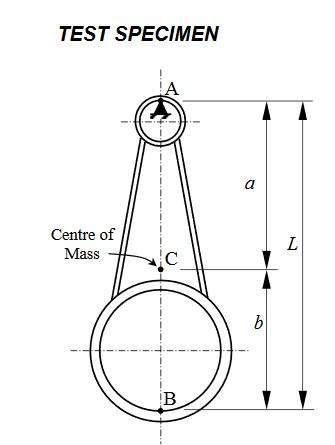
\includegraphics[width=0.5\textwidth]{chapters/lab1/m1}
\caption{Experimental setup for compound pendulum method.}
\label{fig:mesh2}
\end{figure}